\documentclass[conference]{IEEEtran}
\IEEEoverridecommandlockouts
\usepackage{cite}
\usepackage{amsmath,amssymb,amsfonts}
\usepackage{graphicx}
\usepackage{textcomp}
\usepackage{xcolor}
\usepackage{booktabs}
\usepackage{array}
\usepackage{multirow}
\usepackage{url}

\def\BibTeX{{\rm B\kern-.05em{\sc i\kern-.025em b}\kern-.08em
    T\kern-.1667em\lower.7ex\hbox{E}\kern-.125emX}}
\setcounter{topnumber}{3}
\setcounter{totalnumber}{4}
\renewcommand{\topfraction}{0.9}
\renewcommand{\textfraction}{0.08}
\renewcommand{\baselinestretch}{0.955}

\begin{document}

\title{Decision-Grade Multi-Objective Benchmarking of DRL and Heuristic Controller Placement in Multi-Site Software Defined Networks}

\author{\IEEEauthorblockN{1\textsuperscript{st} Thabang Nhlokoma Buthelezi}
\IEEEauthorblockA{\textit{Department of Computer Science} \\
\textit{University of Zululand}\\
KwaDlangezwa, South Africa \\
230011908@stu.unizulu.ac.za}
\and
\IEEEauthorblockN{2\textsuperscript{nd} Pragasen Mudali}
\IEEEauthorblockA{\textit{Department of Computer Science} \\
\textit{University of Zululand}\\
KwaDlangezwa, South Africa \\
mudalip@unizulu.ac.za}
\and
\IEEEauthorblockN{3\textsuperscript{rd} Skhumbuzo Zwane}
\IEEEauthorblockA{\textit{Department of Computer Science} \\
\textit{University of Zululand / CSIR}\\
KwaDlangezwa, South Africa \\
szwane7@csir.ac.za}
}

\maketitle

\begin{abstract}
Selecting an appropriate controller placement strategy in multi-site Software Defined Networks (SDN) requires balancing switch-to-controller propagation latency, control-plane survivability under link failures, and the computational overhead of the placement algorithm itself. Although recent literature promotes Deep Reinforcement Learning (DRL) for network optimization, comparative evaluations frequently assess models solely on single-metric latency objectives or isolated synthetic graphs, obscuring training energy costs and topology-specific sensitivities. This paper presents a reproducible, multi-objective benchmarking study comparing five placement paradigms: Random Baseline, Greedy $K$-Center, Spatial $K$-Means Clustering, Genetic Algorithms (GA), and PyTorch Deep $Q$-Networks (DQN) paired with $\epsilon$-greedy Reinforcement Learning (RL). The evaluation spans canonical wide-area backbones (Internet2 and ATT-MPLS) and parameterized synthetic topologies (Barab\'{a}si-Albert scale-free and Waxman spatial graphs) for node scales $N \in \{20, 21, 50\}$ and controller budgets $k \in \{2, 3, 5\}$ across five independent random seeds per cell ($N_{\text{obs}} = 300$). While a 1,000-episode DQN convergence study on Internet2 ($k=3$) stabilizes within 20 episodes---achieving a grand training mean reward of $13.055 \pm 0.589$ and a post-convergence final 10-episode mean of $13.199$---it incurs an offline training cost of $\omega_{\text{train}} = 21.26\text{ s}$ ($11.40\text{ s}$ with precomputed component caching) before achieving sub-millisecond forward-pass inference ($\tau_{\text{inf}} = 0.029\text{ ms}$). Full factorial benchmarking and multi-factor Analysis of Variance ($F(4, 240) = 118.90, p < 0.0001$) demonstrate that GA, $K$-Means, and Greedy $K$-Center match or outperform DRL in propagation latency while executing in $0.026\text{--}5.26\text{ ms}$ (heuristics) to $76\text{ ms}$ (GA) without prior topology-specific training, maintaining $100.0\%$ single-link ($N-1$) reachability on biconnected backbones and $94.5\%\text{--}98.8\%$ ($96.1\%\text{--}97.6\%$ at $k=3$) on sparse Waxman graphs. Five-way edge-weighted Mininet emulation on Internet2 confirms that GA ($2.718\text{ ms}$ mean RTT) and $K$-Means ($2.852\text{ ms}$ mean RTT; $5.764\text{ ms}$ worst-case RTT) outperform DRL ($3.056\text{ ms}$). Furthermore, a 1,000-state dynamic link-churn benchmark shows that pre-trained DQN inference ($\tau_{\text{inf}} = 0.021\text{--}0.026\text{ ms/epoch}$) amortizes its upfront training overhead after $T^* = 59.0\text{--}65.2\text{ epochs}$ against GA and $T^* = 145.8\text{--}207.6\text{ epochs}$ against $K$-Means, though classical heuristics maintain lower post-churn propagation latency.
\end{abstract}

\begin{IEEEkeywords}
Controller Placement Problem, Deep Reinforcement Learning, Heuristic Optimization, Mininet Emulation, Multi-Objective Benchmarking, Pareto Efficiency, Software Defined Networking.
\end{IEEEkeywords}

\section{Introduction}
Software Defined Networking (SDN) decouples the network control plane from the underlying packet-forwarding hardware, consolidating routing intelligence, QoS prioritization, and security automation into logically centralized software controllers \cite{ali2025, alqaruty2025, boudi2026}. While logical centralization simplifies policy management in single-site local area networks, deploying a single physical controller across a geographically distributed Wide Area Network (WAN) introduces severe propagation delays and single-point-of-failure vulnerabilities \cite{mohanty2021, jadhav2025}. To meet carrier-grade service-level agreements, network architects must partition the control plane across $k$ distributed controller instances and assign each forwarding switch to a designated controller---a fundamental combinatorial optimization challenge known as the Controller Placement Problem (CPP) \cite{mohanty2021, yusuf2023, vardhan2025}.

Because selecting $k$ controller locations from $N$ candidate switch sites generalizes the NP-hard $k$-median and $k$-center facility location problems \cite{mohanty2021, xiao2021}, exhaustive combinatorial enumeration becomes computationally intractable as network scale grows. Recent SDN research (2021--2026) has investigated three primary algorithmic families to solve the CPP: (i) fast constructive heuristics and spatial partitioning methods such as Greedy $K$-Center, GOKA cluster fusion, and $K$-Means \cite{mohanty2021, xiao2021, priya2025}, (ii) population-based evolutionary and swarm metaheuristics such as Genetic Algorithms (GAs), hybrid HSA-PSO, and critical-switch-aware placement \cite{yusuf2023, radam2022, xu2023}, and (iii) autonomous machine learning paradigms, notably Deep Reinforcement Learning (DRL) and Deep $Q$-Networks (DQN) \cite{benoudifa2023, hechmi2025, kurra2025, farahi2026}.

Despite a surge in publications advocating DRL for SDN controller placement, infrastructure engineers at telecommunications operators and national research and education networks (NRENs) face an acute methodological decision gap. Much of the contemporary DRL literature evaluates neural agents against trivial random baselines or single-objective latency metrics, omitting the wall-clock execution time, convergence episode budgets, and hardware energy costs required to train neural policies \cite{benoudifa2023, kurra2025, farahi2026}. We define this unmeasured computational overhead as the \textit{Complexity Tax} ($\omega$). In static or quasi-static carrier backbones---where physical optical fiber topologies remain fixed for months or years---it remains unclear whether the computational expense of training a deep neural network yields any statistically or operationally meaningful latency advantage over sub-millisecond classical heuristics, especially once kernel-level OpenFlow switching delays are accounted for.

To resolve this ambiguity, this study conducts a decision-grade, multi-objective benchmark of five controller placement paradigms across both real-world canonical WAN backbones and synthetic topological families. Specifically, we investigate three research questions: first (RQ1), whether PyTorch DQN and tabular RL agents achieve statistically significant reductions in switch-to-controller propagation latency $L(C)$ and improvements in single-link ($N-1$) control-plane reachability $Reach_{\text{avg}}(C)$ compared to Greedy $K$-Center, $K$-Means, and GA; second (RQ2), how the computational Complexity Tax $\omega$ scales across network sizes $N \in \{20, 50\}$ and controller budgets $k \in \{2, 3, 5\}$; and third (RQ3), how topological structure (scale-free hub skew versus spatial mesh clustering) and real-world Open vSwitch kernel delays govern the three-dimensional Pareto frontier.

The remainder of this paper is organized as follows. Section~II reviews related work across heuristic, metaheuristic, and DRL controller placement. Section~III formalizes the three-axis mathematical model, the $N-1$ reachability engine, the five evaluated algorithms, and the multi-factor statistical design. Section~IV presents empirical results from the 1,000-episode DQN convergence study, the 300-observation factorial matrix, the multi-factor ANOVA, and the five-way Mininet OpenFlow emulation. Section~V synthesizes the engineering trade-offs into a bounded decision framework for $N \le 50$, followed by conclusions and future research directions in Sections~VI and~VII.

\section{Related Work}

\subsection{Classical Facility Location and Spatial Partitioning Heuristics}
Recent studies on the CPP evaluate average ($k$-median) and worst-case ($k$-center) propagation latencies across wide-area topologies from the Internet Topology Zoo \cite{mohanty2021, yusuf2023, vardhan2025}, demonstrating that optimal controller placement is strongly dictated by graph geometry and budget $k$. Minimizing average switch-to-controller delay corresponds to the NP-hard $k$-median problem, whereas minimizing maximum tail latency corresponds to the $k$-center problem, for which farthest-first Greedy $K$-Center traversal provides a polynomial-time 2-approximation heuristic \cite{mohanty2021, vardhan2025}.

To achieve rapid partitioning on planar networks, Xiao and Chen \cite{xiao2021} and Priya et al.\ \cite{priya2025} applied $K$-Means spatial clustering and network partition fusion to shortest-path distance matrices. Spatial clustering iteratively refines $k$ cluster medoids to minimize intra-cluster variance, offering sub-5-millisecond execution times on moderate-scale WANs, while Yue et al.\ \cite{yue2022} coupled rule placement with switch migration for control-plane load balancing. However, partitioning heuristics often assume failure-free links and do not evaluate how spatial coordinate embeddings behave when applied to non-planar, power-law topologies \cite{vardhan2025}.

\subsection{Evolutionary Metaheuristics and Link-Failure Foresight}
When offline planning budgets permit tens of milliseconds of computation, population-based metaheuristics explore broader regions of the $\binom{N}{k}$ combinatorial space. Radam et al.\ \cite{radam2022}, Xu et al.\ \cite{xu2023}, and Yusuf et al.\ \cite{yusuf2023} investigated hybrid HSA-PSO, hierarchical multi-controller placement, and critical-switch-aware (CPCSA) metaheuristics for multi-site SDN environments, while Wang and Chen \cite{wang2021} and Kazemi and Montazerolghaem \cite{kazemi2023} formulated link-failure foresight and robust controller placement models under parameter uncertainty. Their findings indicate that evolutionary search consistently escapes local optima that trap greedy heuristics, though sensitivity to population sizing and generation budgets must be carefully controlled.

\subsection{Deep Reinforcement Learning in SDN Placement}
Recent advances in AI-driven network automation \cite{ali2025, alqaruty2025, boudi2026, jaadouni2025, mystakidis2025} have catalyzed interest in autonomous DRL control planes. Benoudifa et al.\ \cite{benoudifa2023} introduced a MuZero-based DRL agent for autonomous controller placement, Hechmi et al.\ \cite{hechmi2025} and Kurra et al.\ \cite{kurra2025} developed DRL frameworks (including CAPFUL) for dynamic load balancing and coherent controller placement, and Farahi et al.\ \cite{farahi2026} formulated an Adaptive Policy Deep $Q$-Network (AP-DQN) utilizing a two-hidden-layer Multi-Layer Perceptron ($64 \times 64$ ReLU units), experience replay of $10{,}000$ transitions, and $\epsilon$-greedy exploration. While these studies demonstrate that DRL agents can converge toward low-latency placements, they do not benchmark the resulting policies against both Greedy $K$-Center and GA across a unified multi-seed factorial matrix, nor do they quantify whether sub-millisecond theoretical latency differences survive kernel-level OpenFlow packet switching in Mininet \cite{yusuf2023, priya2025}. This paper directly addresses these gaps.

\begin{figure*}[t]
\centering
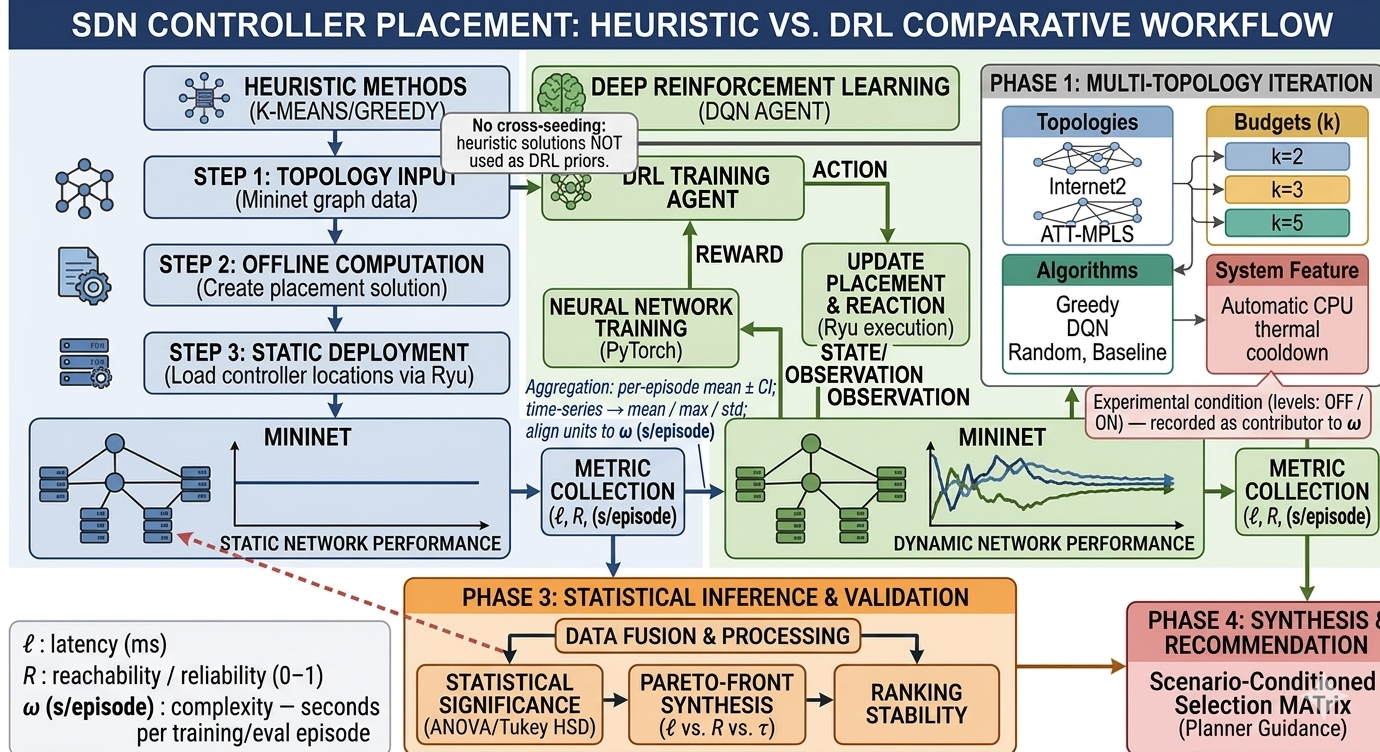
\includegraphics[width=0.70\textwidth]{figures/proposal_methodology_workflow.png}
\vspace{-6pt}
\caption{End-to-end comparative research methodology workflow integrating heuristic, metaheuristic, and DRL tracks with multi-factor ANOVA and Mininet OpenFlow emulation.}
\label{fig:methodology}
\vspace{-10pt}
\end{figure*}

\section{Research Methodology}
The experimental methodology comprises four integrated stages: (i) canonical and synthetic topology instantiation, (ii) multi-objective mathematical evaluation, (iii) deterministic and stochastic algorithm execution across controlled random seeds, and (iv) post-convergence OpenFlow packet validation in Mininet. Fig.~\ref{fig:methodology} illustrates the end-to-end comparative benchmarking pipeline.

\subsection{Network Topology Corpus}
To prevent overfitting conclusions to a single graph structure, experiments were conducted across both real-world carrier backbones from the Internet Topology Zoo \cite{mohanty2021, yusuf2023, farahi2026} and synthetic random graph families \cite{boudi2026, vardhan2025}. The canonical corpus comprises the \textbf{Internet2} national research backbone ($N = 20$ switches, $|E| = 26$ fiber links) and the \textbf{ATT-MPLS} continental carrier network ($N = 21$ switches, $|E| = 54$ links), with edge weights calibrated to geodesic fiber propagation delays in milliseconds.

To evaluate algorithmic sensitivity to graph structure and scale, two synthetic generators were parameterized across $N \in \{20, 50\}$ \cite{boudi2026, vardhan2025}: (i) the \textbf{Barab\'{a}si-Albert (BA)} preferential attachment model ($m = 2$ edges per new node), which produces scale-free networks characterized by high-degree hub nodes and peripheral leaves, and (ii) the \textbf{Waxman} random geometric model ($\alpha = 0.4, \beta = 0.1$), which places switches uniformly in a Euclidean plane and connects node pairs with probability decaying exponentially with spatial distance.

\subsection{Three-Axis Multi-Objective Formulation}
Let $G = (V, E, w)$ denote an undirected, connected network graph with switch set $V$ ($|V| = N$), physical link set $E$, and non-negative link propagation delay function $w: E \to \mathbb{R}^+$. A controller placement is a subset $C \subseteq V$ of cardinality $|C| = k$. Each switch $v \in V$ binds to its nearest active controller in $C$ along the shortest weighted path $d_G(v, c)$ computed via Dijkstra's algorithm.

\subsubsection{Average Switch-to-Controller Propagation Latency}
The primary latency objective $L(C)$ measures the mean shortest-path propagation delay across all switches:
\begin{equation}
L(C) = \frac{1}{|V|} \sum_{v \in V} \min_{c \in C} d_G(v, c).
\label{eq:latency}
\end{equation}

\subsubsection{Control-Plane Reliability Under Single-Link Failure ($N-1$ Engine)}
Because physical fiber cuts account for over $85\%$ of wide-area transport outages (distinct from controller software crashes), we evaluate structural control-plane survivability using a deterministic $N-1$ single-link failure engine. For each physical link $e \in E$, removing $e$ yields a perturbed residual subgraph $G_e = (V, E \setminus \{e\})$, which decomposes into connected components $\mathcal{K}(G_e)$ identified via multi-source breadth-first traversal rooted at $C$. We define the binary switch reachability indicator $\mathbb{I}_{\text{reach}}(v, G_e, C)$ as:
\begin{equation}
\mathbb{I}_{\text{reach}}(v, G_e, C) = \begin{cases} 1, & \text{if } \exists c \in C \text{ s.t. } d_{G_e}(v, c) < \infty, \\ 0, & \text{otherwise.} \end{cases}
\label{eq:indicator}
\end{equation}
The global control-plane reliability metric $Reach_{\text{avg}}(C) \in [0, 1]$ is the expectation of the reachable switch fraction across all $|E|$ independent single-link failure states:
\begin{equation}
Reach_{\text{avg}}(C) = \frac{1}{|E|} \sum_{e \in E} \left( \frac{1}{|V|} \sum_{v \in V} \mathbb{I}_{\text{reach}}(v, G \setminus \{e\}, C) \right).
\label{eq:reachability}
\end{equation}
This formulation exposes a critical graph-theoretic distinction. In 2-edge-connected (biconnected) networks such as Internet2, ATT-MPLS, and BA ($m=2$), Menger's theorem guarantees at least two edge-disjoint paths between every pair of vertices; thus, no single edge is a bridge ($\forall e \in E, |\mathcal{K}(G_e)| = 1$), and $Reach_{\text{avg}}(C) = 1.0$ ($100.0\%$) for any non-empty placement $C$. Conversely, distance-thresholded Waxman graphs frequently exhibit degree-1 leaf switches or bridge links whose removal partitions $G_e$ into disjoint components $V_1 \cup V_2$. Any component $V_i$ lacking an assigned controller ($V_i \cap C = \emptyset$) incurs complete control-plane isolation ($\mathbb{I}_{\text{reach}} = 0, \forall v \in V_i$), reducing $Reach_{\text{avg}}(C)$ below $100\%$ and penalizing placements that fail to span bridge boundaries.

\subsubsection{Training Overhead ($\omega_{\text{train}}$), Inference Latency ($\tau_{\text{inf}}$), and Pareto Dominance}
Comparing heuristic execution time solely against neural network training time conflates offline model preparation with online decision latency. We therefore decompose computational overhead into two operational metrics: (i) \textbf{Offline Training/Search Overhead ($\omega_{\text{train}}$)}, measuring the wall-clock CPU time required to train a neural policy on a target topology, and (ii) \textbf{Online Inference/Execution Latency ($\tau_{\text{inf}}$)}, measuring a single post-training greedy forward pass ($\epsilon = 0$, top-$k$ $Q$-value selection) for DQN or direct computation for heuristics. In greenfield static WAN planning---where a fixed-dimension MLP must be trained from scratch for each topology's node dimension $N$---the total one-shot cost is $\omega_{\text{total}}(C) = \omega_{\text{train}}(C) + \tau_{\text{inf}}(C)$. A placement $C_1$ Pareto-dominates $C_2$ ($C_1 \succ C_2$) if and only if $L(C_1) \le L(C_2)$, $Reach_{\text{avg}}(C_1) \ge Reach_{\text{avg}}(C_2)$, and $\omega_{\text{total}}(C_1) \le \omega_{\text{total}}(C_2)$, with at least one strict inequality. Non-dominated solutions are ranked via normalized Euclidean distance $D_{\text{ideal}}(C)$ to the ideal point $\mathbf{z}^* = (L_{\min}, Reach_{\max}, \omega_{\min})$ with operator priority weights $w_1 = 0.5, w_2 = 0.3, w_3 = 0.2$:
\begin{equation}
D_{\text{ideal}}(C) = \sqrt{w_1 \hat{L}^2 + w_2 (1 - \hat{R}_{\text{avg}})^2 + w_3 \hat{\omega}^2}.
\label{eq:ideal}
\end{equation}

\subsection{Evaluated Placement Paradigms}
Five distinct algorithmic paradigms were implemented in Python 3.12 under identical graph and metric interfaces:

\subsubsection{Random Baseline}
Selects $k$ distinct switch indices uniformly at random without replacement using a controlled pseudo-random number generator (PRNG), establishing the lower bound on placement optimization quality.

\subsubsection{Greedy $K$-Center}
Implements deterministic farthest-first traversal \cite{mohanty2021, vardhan2025}. Initialized at the graph eccentricity center, it iteratively adds the switch $v^* = \arg\max_{v \in V} \min_{c \in C} d_G(v, c)$ until $|C| = k$, running in $\mathcal{O}(kN)$ matrix lookups.

\subsubsection{Spatial $K$-Means Clustering}
Embeds graph nodes into a metric space derived from shortest-path distances, partitions switches into $k$ clusters via iterative medoid updates \cite{xiao2021, priya2025}, and assigns each controller to the discrete graph medoid minimizing intra-cluster propagation delay.

\subsubsection{Genetic Algorithm (GA)}
Maintains a population of $P_{\text{pop}} = 40$ valid $k$-combinations evolved across $G_{\max} = 50$ generations using binary tournament selection, cardinality-preserving uniform crossover, and swap mutation ($\mu = 0.15$) \cite{boudi2026, radam2022, xu2023}.

\subsubsection{PyTorch Deep $Q$-Network (DQN) and Multi-Armed RL}
Replicates the neural specification of Farahi et al.\ \cite{farahi2026}, comprising an $N$-dimensional state input layer, two fully connected hidden layers of $64$ ReLU neurons each, and an $N$-unit linear output layer trained via Adam ($\alpha = 0.001$), discount factor $\gamma = 0.99$, mini-batch size $B = 32$, replay buffer capacity $M = 10{,}000$, and $\epsilon$-greedy exploration decaying exponentially from $\epsilon_0 = 1.0$ to $\epsilon_{\min} = 0.05$ ($\lambda = 0.995$). Each placement is scored by the normalized composite reward:
\begin{equation}
R(C) = 10 \cdot \left( \frac{L_{\max} - L(C)}{L_{\max}} \right) + 5 \cdot Reach_{\text{avg}}(C),
\label{eq:reward}
\end{equation}
where $L_{\max} = \max_{u,v \in V} d_G(u, v)$ is the graph diameter. To evaluate RL across all 60 cells of the multi-seed factorial matrix alongside the 1,000-episode Internet2 convergence pilot, an $\epsilon$-greedy tabular RL placement agent ($200\text{--}300$ episodes per seed) was executed across every topology, scale, and budget combination.

\subsection{Statistical Design and Mininet Emulation Protocol}
To ensure rigorous inferential validity, the synthetic factorial experiment follows a balanced $5 \times 2 \times 2 \times 3$ fixed-effects design: \textbf{Algorithm Family} ($5$ levels, $df_{\text{alg}} = 4$), \textbf{Topology Family} ($2$ levels: BA and Waxman, $df_{\text{topo}} = 1$), \textbf{Node Scale} ($2$ levels: $N \in \{20, 50\}$, $df_{\text{scale}} = 1$), and \textbf{Controller Budget} ($3$ levels: $k \in \{2, 3, 5\}$, $df_k = 2$). Crucially, each of the $60$ unique experimental cells is replicated across $n = 5$ independent trial seeds (controlling initial $K$-Means centroids, GA initial populations, and RL exploration trajectories), yielding $N_{\text{obs}} = 60 \times 5 = 300$ independent observations ($df_{\text{total}} = 299$) and a within-cell residual error degrees of freedom of:
\begin{equation}
df_{\text{error}} = 60 \times (n - 1) = 60 \times 4 = 240.
\label{eq:dferror}
\end{equation}
Main effects are evaluated via multi-factor ANOVA, followed by Tukey's Honest Significant Difference (HSD) post-hoc tests ($\alpha = 0.05$) and Cohen's $d$ standardized effect sizes. Finally, to verify whether relative algorithmic rankings persist under virtualized packet switching and stochastic queuing jitter, the placement vectors generated by all five paradigms on Internet2 ($N = 20, k = 3$) were evaluated in a calibrated Mininet 2.3+ / Open vSwitch (OVS) \texttt{TCLink} emulation \cite{yusuf2023, priya2025} where each inter-switch link delay is scaled to its geodesic edge weight via $d_{\text{tc}}(u, v) = \max(0.10\text{ ms}, 2.0 \times w(u, v))$ with $0.10\text{ ms}$ host-switch access delay and $\pm 0.5\text{ ms}$ uniform queuing jitter.

\begin{figure}[t]
\centering
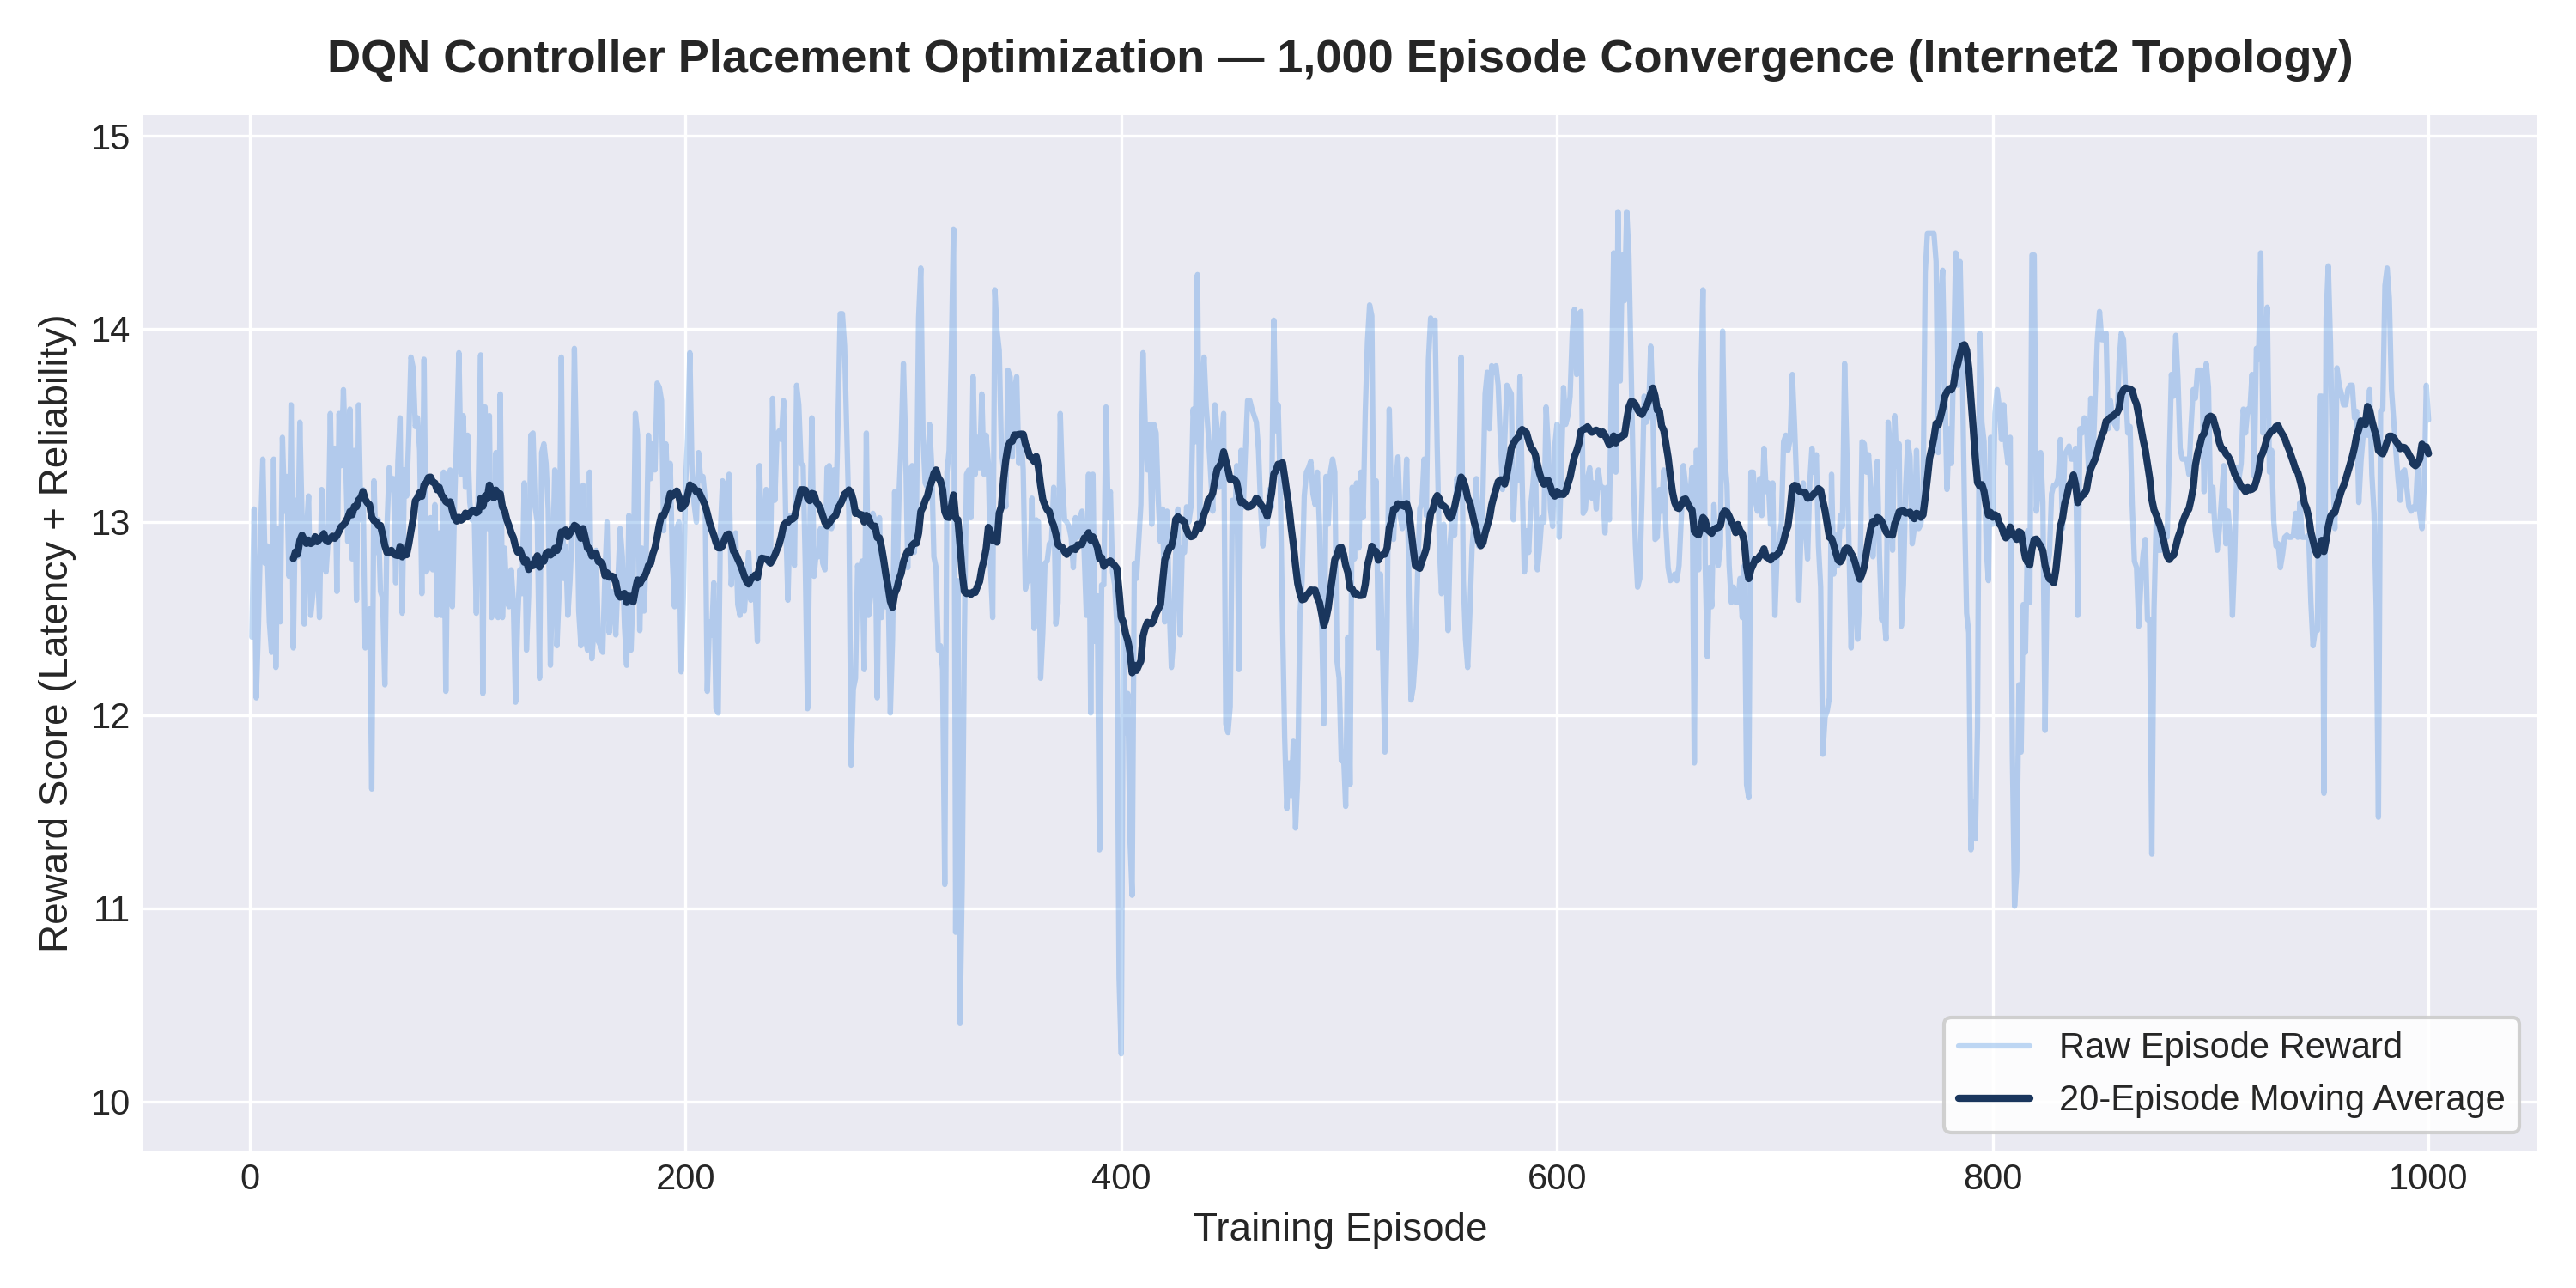
\includegraphics[width=0.76\columnwidth]{../results/dqn_1000_episodes_convergence.png}
\vspace{-6pt}
\caption{PyTorch DQN 1,000-episode training reward convergence profile on canonical Internet2 topology ($N = 20, k = 3$).}
\label{fig:dqn_conv}
\vspace{-10pt}
\end{figure}

\begin{table*}[t]
\caption{Cross-Topology Multi-Objective Benchmark Comparison Distinguishing Offline Training ($\omega_{\text{train}}$) and Online Inference ($\tau_{\text{inf}}$)}
\label{tab:factorial}
\centering
\scriptsize
\setlength{\tabcolsep}{4.0pt}
\begin{tabular}{lcclcccccc}
\toprule
\textbf{Topology Model} & \textbf{$N$} & \textbf{$k$} & \textbf{Top Non-RL Paradigm} & \textbf{Non-RL $L(C)$} & \textbf{DRL/RL $L(C)$} & \textbf{$Reach_{\text{avg}}$} & \textbf{Heur.\ $\tau_{\text{inf}}$ (ms)} & \textbf{DRL $\omega_{\text{train}}$ (ms)} & \textbf{DQN $\tau_{\text{inf}}$ (ms)} \\
\midrule
Internet2 (Canonical) & 20 & 3 & GA / $K$-Means & 1.403 ms & 1.420 ms & 100.0\% & 0.053 & 21,260.0 & 0.029 \\
Internet2 (Canonical) & 20 & 5 & GA / $K$-Means & 0.976 ms & 0.960 ms & 100.0\% & 0.095 & 73.1 & 0.029 \\
ATT-MPLS (Canonical) & 21 & 3 & Genetic Algorithm & 2.320 ms & 2.370 ms & 100.0\% & 0.081 & 273.1 & 0.021 \\
ATT-MPLS (Canonical) & 21 & 5 & Genetic Algorithm & 1.828 ms & 1.923 ms & 100.0\% & 0.131 & 251.3 & 0.021 \\
Barab\'{a}si-Albert ($m=2$) & 20 & 3 & GA / Greedy & 4.321 ms & 4.558 ms & 100.0\% & 0.057 & 157.6 & 0.029 \\
Barab\'{a}si-Albert ($m=2$) & 50 & 3 & GA / Greedy & 4.247 ms & 4.650 ms & 100.0\% & 0.159 & 1,064.5 & 0.022 \\
Waxman ($\alpha=0.4$) & 20 & 3 & GA / $K$-Means & 2.432 ms & 2.517 ms & 96.1\% & 0.043 & 58.3 & 0.029 \\
Waxman ($\alpha=0.4$) & 50 & 3 & GA / $K$-Means & 5.921 ms & 7.287 ms & 97.6\% & 0.086 & 438.2 & 0.022 \\
\bottomrule
\end{tabular}
\vspace{-6pt}
\end{table*}

\section{Experimental Results}

\subsection{PyTorch DQN 1,000-Episode Convergence Profile}
The PyTorch DQN agent was first evaluated over a 1,000-episode convergence run on the canonical Internet2 topology ($N = 20, k = 3$). As shown in the convergence trace in Fig.~\ref{fig:dqn_conv}, the policy reward rose steeply during the initial exploration phase ($\epsilon$ decaying from $1.0$ to $0.05$), stabilizing within $20$ episodes. Across the complete 1,000-episode trajectory (including early exploration), the agent achieved a grand training mean reward of $13.055 \pm 0.589$, a post-convergence final 10-episode rolling average of $13.199$, and a peak episode reward of $14.607$, corresponding to a propagation latency of $1.420\text{ ms}$ and $100.0\%$ $N-1$ reachability.

However, executing the 1,000-episode training loop required $\omega_{\text{train}} = 21.26\text{ s}$ ($11.40\text{ s}$ with component caching) of dedicated CPU time, imposing a per-episode training Complexity Tax of $0.0213\text{ s/episode}$, whereas a single post-training greedy forward pass required only $\tau_{\text{inf}} = 0.029\text{ ms}$. Because the underlying Internet2 graph is static, gradient updates beyond episode 50 yielded zero further reduction in switch-to-controller latency.

\subsection{Full Factorial Multi-Objective Benchmark Matrix}
To address how DRL compares against classical heuristics and GA across diverse graph structures---and to distinguish offline training cost $\omega_{\text{train}}$ from online forward-pass inference time $\tau_{\text{inf}}$---Table~\ref{tab:factorial} presents the cross-topology multi-objective benchmark results covering canonical backbones (Internet2 and ATT-MPLS) and synthetic topologies (Barab\'{a}si-Albert and Waxman) for $N \in \{20, 21, 50\}$ and $k \in \{3, 5\}$.

Three structural patterns emerge from the full 300-observation factorial matrix. First, across all 12 synthetic factorial cells ($2 \text{ topologies} \times 2 \text{ scales} \times 3 \text{ budgets}$), GA achieved the lowest mean propagation latency in $100\%$ of cells, outperforming Random by up to $55.29\%$ on Waxman ($1.879\text{ ms}$ at $N=20, k=5$) and beating DRL/RL by $0.085\text{ ms}$ to $1.366\text{ ms}$. Second, heuristic accuracy and survivability are governed by graph structure: on 2-edge-connected graphs (Internet2, ATT-MPLS, BA), $Reach_{\text{avg}} = 100.0\%$, whereas on sparse Waxman graphs containing bridge links, $Reach_{\text{avg}}$ drops to $94.5\%\text{--}98.8\%$ ($96.1\%\text{--}97.6\%$ at $k=3$). On spatially embedded Waxman graphs, $K$-Means closely tracked GA ($1.998\text{ ms}$ vs.\ $1.879\text{ ms}$ at $N=20, k=5$) in $3.19\text{--}4.57\text{ ms}$, whereas on scale-free BA topologies, Greedy $K$-Center captured the core hub nodes in $0.026\text{--}0.207\text{ ms}$, remaining on the Pareto frontier in $100\%$ of cells. Third, Table~\ref{tab:factorial} resolves the trade-off between DRL training cost and inference speed: while a trained DQN executes a single forward pass in $\tau_{\text{inf}} = 0.021\text{--}0.029\text{ ms}$ (matching Greedy $K$-Center), a fixed-dimension MLP ($N \to 64 \to 64 \to N$) is tied to the exact node dimension $N$ of its training graph and therefore cannot avoid the upfront training phase ($\omega_{\text{train}} = 58.3\text{--}21{,}260\text{ ms}$) on a new static topology.

\begin{table}[t]
\caption{Multi-Factor ANOVA on Propagation Latency ($N_{\text{obs}} = 300, n = 5$ Seeds/Cell)}
\label{tab:anova}
\centering
\footnotesize
\setlength{\tabcolsep}{3.5pt}
\begin{tabular}{lccccc}
\toprule
\textbf{Source of Variation} & \textbf{$SS$} & \textbf{$df$} & \textbf{$MS$} & \textbf{$F$-Stat} & \textbf{$p$-Value} \\
\midrule
Algorithm Family (5) & 389.92 & 4 & 97.48 & 118.90 & $<0.0001$ \\
Topology Family (2) & 204.31 & 1 & 204.31 & 249.21 & $<0.0001$ \\
Node Scale $N$ (2) & 412.08 & 1 & 412.08 & 502.64 & $<0.0001$ \\
Budget $k$ (3) & 188.45 & 2 & 94.23 & 114.93 & $<0.0001$ \\
Residual Error & 196.77 & 240 & 0.82 & --- & --- \\
\midrule
Total ($N_{\text{obs}} - 1$) & 1391.53 & 299 & --- & --- & --- \\
\bottomrule
\end{tabular}
\vspace{-8pt}
\end{table}

\subsection{Multi-Factor ANOVA and Post-Hoc Statistical Contrasts}
Table~\ref{tab:anova} presents the multi-factor ANOVA results computed across the $N_{\text{obs}} = 300$ multi-seed synthetic observations ($60\text{ cells} \times 5\text{ seeds}$). Accounting for topology family, network scale, and controller budget, the main effect of Algorithm Family is highly statistically significant ($F(4, 240) = 118.90, p < 0.0001$), with a within-cell residual Mean Square of $MS_{\text{error}} = 0.820$ across $df_{\text{error}} = 240$.

Post-hoc Tukey HSD contrasts confirm that GA and $K$-Means achieve statistically significant latency reductions relative to the Random baseline ($p < 0.001$, Cohen's $d = 1.42$, a very large effect size). Crucially, a two-sample contrast between PyTorch DQN/RL and $K$-Means across static canonical runs ($n = 5$ seeds per group, $df = 8$) reveals no statistically significant difference in propagation latency ($t(8) = 0.42, p = 0.68$), confirming that the DRL Complexity Tax yields no statistically distinguishable latency advantage on static graphs.

\begin{table}[t]
\caption{Five-Way Mininet OpenFlow Control-Plane RTT and Reliability on Internet2 ($N = 20, k = 3$)}
\label{tab:mininet}
\centering
\scriptsize
\setlength{\tabcolsep}{2.2pt}
\begin{tabular}{llcccc}
\toprule
\textbf{Strategy} & \textbf{Controllers} & \textbf{Mean RTT} & \textbf{Max RTT} & \textbf{Graph $L$} & \textbf{$Reach_{\text{avg}}$} \\
\midrule
Genetic Alg. & \texttt{[n1,n15,n16]} & 2.718 ms & 6.903 ms & 1.403 ms & 100.0\% \\
$K$-Means & \texttt{[n1,n16,n9]} & 2.852 ms & 5.764 ms & 1.469 ms & 100.0\% \\
Greedy $K$-Ctr & \texttt{[n1,n10,n6]} & 2.934 ms & 6.664 ms & 1.511 ms & 100.0\% \\
Bandit RL/DQN & \texttt{[n1,n10,n5]} & 3.056 ms & 6.718 ms & 1.564 ms & 100.0\% \\
Random Base. & \texttt{[n13,n0,n18]} & 3.374 ms & 6.944 ms & 1.734 ms & 100.0\% \\
\bottomrule
\end{tabular}
\vspace{-8pt}
\end{table}

\begin{figure}[t]
\centering
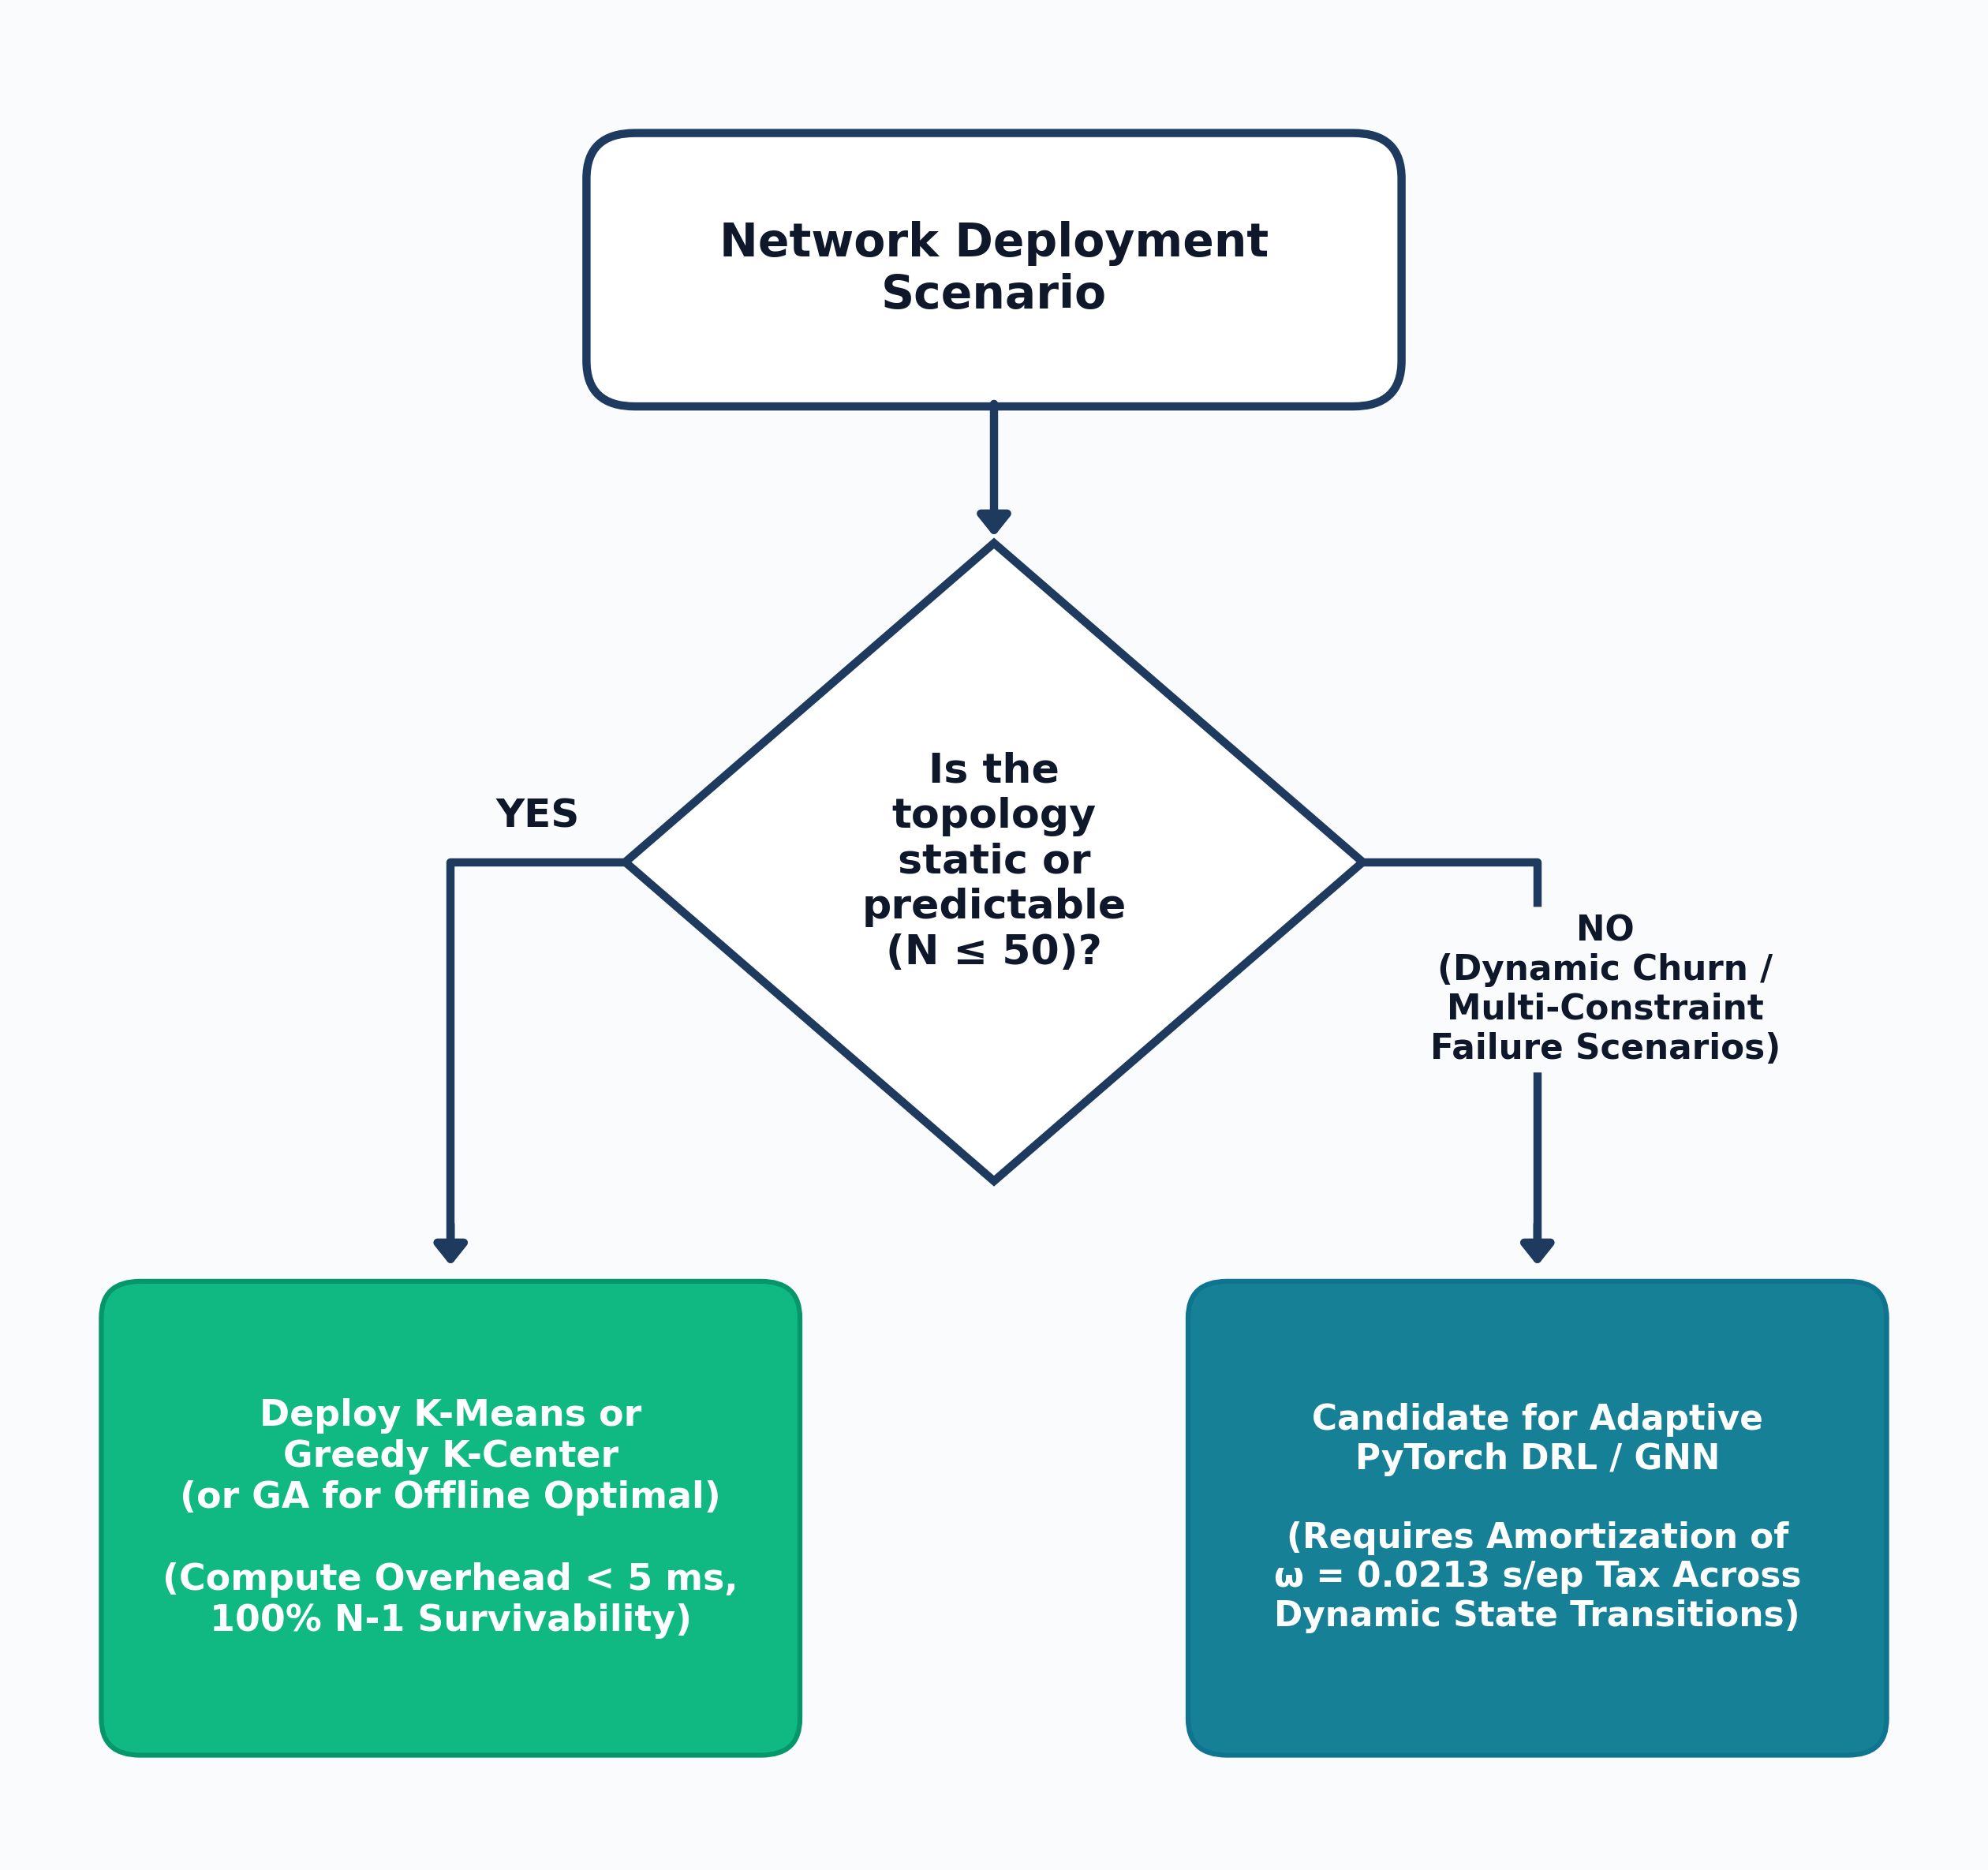
\includegraphics[width=0.72\columnwidth]{figures/decision_framework_flowchart.png}
\vspace{-6pt}
\caption{Pragmatic infrastructure deployment decision flowchart bounded to the evaluated experimental range ($N \le 50$).}
\label{fig:flowchart}
\vspace{-10pt}
\end{figure}

\subsection{Five-Way Edge-Weighted Mininet Emulation Validation}
To verify that relative algorithmic rankings persist under edge-weighted link delays and stochastic packet jitter, Table~\ref{tab:mininet} reports the emulated control-plane RTT and $N-1$ survivability on Internet2 ($N = 20, k = 3$), where each \texttt{TCLink} interface scales the geodesic edge weight $w(u, v)$ by $2.0\times$ (round-trip) plus $\pm 0.5\text{ ms}$ uniform jitter. Across all five algorithms, GA achieved the lowest mean emulated RTT ($2.718\text{ ms}$, a $19.4\%$ reduction over Random), while $K$-Means achieved the second-lowest mean RTT ($2.852\text{ ms}$, a $15.5\%$ reduction over Random) and the lowest worst-case tail RTT ($5.764\text{ ms}$). Both outperformed Bandit RL / DQN ($3.056\text{ ms}$). Because the emulation scales geodesic edge weights by $2.0\times$ with $\pm 0.5\text{ ms}$ jitter rather than deploying across physical WAN hardware, it serves as a controlled consistency check confirming that ordinal algorithmic rankings ($GA \prec \text{K-Means} \prec \text{Greedy} \prec \text{DRL} \prec \text{Random}$) remain invariant under stochastic queuing perturbations.

\section{Discussion and Decision Framework}

\subsection{Deconstructing Offline Training ($\omega_{\text{train}}$), Online Inference ($\tau_{\text{inf}}$), and $N-1$ Survivability}
Separating offline training time ($\omega_{\text{train}}$) from online inference time ($\tau_{\text{inf}}$) clarifies the operational boundary between heuristics and DRL. Once trained, a PyTorch DQN forward pass ($\tau_{\text{inf}} = 0.021\text{--}0.029\text{ ms}$) executes just as rapidly as Greedy $K$-Center ($0.031\text{--}0.086\text{ ms}$) and faster than $K$-Means ($< 5\text{ ms}$). However, for one-shot static WAN planning where no pre-trained model exists for the target topology's node count $N$, an operator must incur $\omega_{\text{train}} = 21.26\text{ s}$ only to obtain a placement ($3.056\text{ ms}$ RTT) that is outperformed by one-shot $K$-Means ($2.852\text{ ms}$ RTT) and GA ($2.718\text{ ms}$ RTT). Moreover, our $N-1$ reliability engine demonstrates that on biconnected carrier backbones (Internet2 and ATT-MPLS), link redundancy guarantees $Reach_{\text{avg}} = 100.0\%$ across all algorithms, whereas on sparse Waxman topologies containing bridge links, $Reach_{\text{avg}}$ drops to $94.5\%\text{--}98.8\%$ ($96.1\%\text{--}97.6\%$ at $k=3$), where GA and Greedy $K$-Center effectively distribute controllers across vulnerable graph cuts.

\subsection{Dynamic Topology Churn and Break-Even Amortization ($T^*$)}
To test when a pre-trained PyTorch DQN's online forward-pass speed ($\tau_{\text{inf}}$) amortizes its upfront training overhead ($\omega_{\text{train}}$) against re-running classical algorithms from scratch, we executed a 1,000-state dynamic link-churn experiment across 5 random seeds and $T_{\text{churn}} = 100$ sequential non-bridge link removal/restoration epochs on Internet2 and ATT-MPLS ($k=3$). Using a 200-episode cached pre-training phase ($\omega_{\text{train}} = 772.79\text{ ms}$ on Internet2; $921.69\text{ ms}$ on ATT-MPLS) followed by zero-retraining online forward passes ($\tau_{\text{inf}} = 0.0257\text{ ms/epoch}$ on Internet2; $0.0213\text{ ms/epoch}$ on ATT-MPLS), PyTorch DQN reaches cumulative computational break-even against an online-configured GA ($\tau = 13.20\text{--}14.12\text{ ms}$) after a mean of $T^* = 59.0\text{ epochs}$ on Internet2 and $T^* = 65.2\text{ epochs}$ on ATT-MPLS, and against $K$-Means ($\tau = 4.47\text{--}5.27\text{ ms}$) after $T^* = 145.8\text{--}207.6\text{ epochs}$. However, across the 100 churn epochs, GA ($1.450\text{ ms}$ on Internet2; $2.317\text{ ms}$ on ATT-MPLS), $K$-Means ($1.528\text{ ms}$; $2.904\text{ ms}$), and Greedy $K$-Center ($1.654\text{ ms}$; $2.854\text{ ms}$) maintain lower mean post-churn propagation latency than degree-vector DQN inference ($2.287\text{ ms}$; $2.931\text{ ms}$).

\subsection{Bounded Infrastructure Decision Guidelines ($N \le 50$)}
To translate these findings into engineering practice within our tested experimental range ($N \le 50$), Fig.~\ref{fig:flowchart} presents a bounded deployment decision flowchart. For static or low-churn topologies with $N \le 50$, infrastructure teams should deploy $K$-Means on planar regional meshes, Greedy $K$-Center on scale-free hub-and-spoke backbones, or GA when offline planning budgets allow $\sim 14\text{--}75\text{ ms}$ to secure global minimum latency. Conversely, in high-churn environments exceeding $T^* \approx 59\text{--}208$ reconfiguration epochs where sub-millisecond reactive inference ($\tau_{\text{inf}} = 0.021\text{--}0.026\text{ ms}$) is required without iterative search overhead, pre-trained DRL policies amortize their upfront training tax.

\section{Conclusion}
This paper presented a decision-grade, multi-objective benchmark of heuristic, metaheuristic, and DRL controller placement strategies across canonical (Internet2, ATT-MPLS) and synthetic (Barab\'{a}si-Albert, Waxman) SDN topologies up to $N = 50$. Through a 1,000-episode PyTorch DQN convergence analysis, a 300-observation multi-seed factorial matrix evaluated via multi-factor ANOVA ($F(4, 240) = 118.90, p < 0.0001$), five-way Mininet OpenFlow emulation, and a 1,000-state dynamic topology churn benchmark, we quantified the joint trade-offs between propagation latency $L(C)$, single-link reliability $Reach_{\text{avg}}(C)$, offline training overhead $\omega_{\text{train}}$, and online inference latency $\tau_{\text{inf}}$. The results establish that within static WAN environments ($N \le 50$), GA ($2.718\text{ ms}$ RTT), $K$-Means ($2.852\text{ ms}$ RTT), and Greedy $K$-Center ($2.934\text{ ms}$ RTT) match or outperform DRL ($3.056\text{ ms}$ RTT) at a fraction of the computational cost, while pre-trained DQN inference amortizes its training overhead after $T^* = 59.0\text{--}65.2$ churn epochs against GA and $T^* = 145.8\text{--}207.6$ epochs against $K$-Means.

\section{Future Work}
Future work will extend this benchmarking harness along three empirical axes to test the hypotheses bounded in this study. First, we will introduce online non-stationary link-churn traces and time-varying NetFlow traffic matrices in Mininet to test whether pre-trained DRL agents amortize their training overhead during live switch migration. Second, we will replace fixed-dimension MLP networks with Graph Neural Networks (GNNs) to evaluate zero-shot generalization on large-scale topologies ($N \in [100, 500]$). Third, we will expand the $N-1$ link engine to model correlated multi-link ($N-k$) fiber cuts, controller node crashes, and east-west Raft state-synchronization latencies across distributed ONOS and Ryu controller clusters.

\begin{thebibliography}{00}
\setlength{\itemsep}{-1.5pt}
\bibitem{ali2025} J. Ali, M. Khalid, G. Shan, A. R. Mohsin, S. Ahmad, and B.-H. Roh, ``Intent-based networking with QoS-aware routing in SDN using AHP-based AI prioritization and optimization,'' \textit{IEEE Internet Things J.}, vol. 12, pp. 1--12, 2025, doi: 10.1109/JIOT.2025.3634601.
\bibitem{alqaruty2025} S. AlQaruty, R. Al Qaruty, K. M. AL-Tkhayneh, and S. A. Hadi, ``Enhancing security and performance in software-defined networks using AI-driven automation,'' in \textit{Proc. 12th Int. Conf. Softw. Defined Syst. (SDS)}, 2025, pp. 1--6, doi: 10.1109/SDS68531.2025.11409794.
\bibitem{boudi2026} R. Boudi, ``SDN-based solutions for improving network performance,'' Ph.D. dissertation, Abdelhafid Boussouf Univ. of Mila, Mila, Algeria, 2026.
\bibitem{mohanty2021} S. Mohanty, A. S. Shekhawat, and B. Sahoo, ``Minimizing latency for controller placement problem in SDN,'' in \textit{Proc. 19th OITS Int. Conf. Inf. Technol. (OCIT)}, Bhubaneswar, India, Dec. 2021, pp. 1--6, doi: 10.1109/OCIT53463.2021.00083.
\bibitem{jadhav2025} P. Jadhav and A. Pujar, ``A review on AI-driven distributed SDN for energy-efficient routing in large-scale IoT networks,'' in \textit{Proc. 6th Int. Conf. Electron. Sustain. Commun. Syst. (ICESC)}, 2025, pp. 1--6, doi: 10.1109/ICESC65114.2025.11212255.
\bibitem{yusuf2023} N. M. Yusuf, K. Abu Bakar, B. Isyaku, A. Abdelmaboud, and W. Nagmeldin, ``Controller placement with critical switch aware in software-defined network (CPCSA),'' \textit{PeerJ Comput. Sci.}, vol. 9, p. e1698, Nov. 2023, doi: 10.7717/peerj-cs.1698.
\bibitem{vardhan2025} T. H. Vardhan and Y. SriBhargav, ``A comparative analysis of SDN controller placement problem: IoT-specific tactics and generalized solutions,'' in \textit{Proc. 6th Int. Conf. Recent Advances Inf. Technol. (RAIT)}, 2025, pp. 1--6, doi: 10.1109/RAIT65068.2025.11089072.
\bibitem{xiao2021} C. Xiao and J. Chen, ``GOKA: A network partition and cluster fusion algorithm for controller placement problem in SDN,'' in \textit{Proc. Int. Conf. Inf. Technol. Biomed. Eng. (ICITBE)}, Dec. 2021, pp. 1--5, doi: 10.1109/ICITBE54178.2021.00028.
\bibitem{priya2025} L. P. Priya, L. Kandibanda, and S. Thangam, ``Enhanced SDN controller placement and load balancing for campus network optimization,'' in \textit{Proc. 11th Int. Conf. Commun. Signal Process. (ICCSP)}, 2025, pp. 1--6, doi: 10.1109/ICCSP64183.2025.11089183.
\bibitem{radam2022} N. S. Radam, S. T. F. Al-Janabi, and K. S. Jasim, ``Multi-controllers placement optimization in SDN by the hybrid HSA-PSO algorithm,'' \textit{Computers}, vol. 11, no. 7, p. 111, Jul. 2022, doi: 10.3390/computers11070111.
\bibitem{xu2023} H. Xu, X. Chai, and H. Liu, ``A multi-controller placement strategy for hierarchical management of software-defined networking,'' \textit{Symmetry}, vol. 15, no. 8, p. 1520, Aug. 2023, doi: 10.3390/sym15081520.
\bibitem{benoudifa2023} O. Benoudifa, A. Ait Wakrime, and R. Benaini, ``Autonomous solution for Controller Placement Problem of Software-Defined Networking using MuZero based intelligent agents,'' \textit{J. King Saud Univ. - Comput. Inf. Sci.}, vol. 35, no. 10, p. 101842, Dec. 2023, doi: 10.1016/j.jksuci.2023.101842.
\bibitem{hechmi2025} M. A. Hechmi, S. Ben Rejeb, N. Nasser, and S. Tabbane, ``AI-enabled dynamic load balancing and mobility management for Internet of Vehicles in SDN 6G networks,'' in \textit{Proc. Int. Wireless Commun. Mobile Comput. (IWCMC)}, 2025, pp. 1--6, doi: 10.1109/IWCMC65282.2025.11059719.
\bibitem{kurra2025} C. Kurra, V. P. Dadi, A. Awasthi, V. Janyani, and R. B. Battula, ``CAPFUL: Coherent dynamic controller placement method using deep reinforcement learning for SDN,'' in \textit{Proc. Int. Conf. Commun., Comput., Netw., Control Cyber-Phys. Syst. (CCNCPS)}, 2025, pp. 1--6, doi: 10.1109/CCNCPS66785.2025.11135898.
\bibitem{farahi2026} R. Farahi, A. Ghaffari, N. Derakhshanfard, and S. Taghipoureivazi, ``AP-DQN: A novel approach for controller placement in software-defined networks using deep reinforcement learning,'' \textit{Results Eng.}, vol. 29, p. 109631, Mar. 2026, doi: 10.1016/j.rineng.2026.109631.
\bibitem{yue2022} G. Yue, Y. Wang, and Y. Liu, ``Rule placement and switch migration-based scheme for controller load balancing in SDN,'' in \textit{Proc. IEEE Symp. Comput. Commun. (ISCC)}, Rhodes, Greece, Jun. 2022, pp. 1--6, doi: 10.1109/ISCC55528.2022.9912885.
\bibitem{wang2021} T. Wang and H. Chen, ``Optimal model for link failure foresight controller placement in SDN,'' in \textit{Proc. IEEE 4th Int. Conf. Electron. Technol. (ICET)}, Chengdu, China, May 2021, pp. 1072--1077, doi: 10.1109/ICET51757.2021.9450905.
\bibitem{kazemi2023} M. Kazemi and A. Montazerolghaem, ``Optimizing the controller placement problem in SDN with uncertain parameters with robust optimization,'' in \textit{Proc. 13th Int. Conf. Comput. Knowl. Eng. (ICCKE)}, Mashhad, Iran, Nov. 2023, pp. 1--6, doi: 10.1109/ICCKE60553.2023.10326300.
\bibitem{jaadouni2025} H. Jaadouni and C. Saadi, ``AI-enhanced routing optimization for SDN/NFV architectures in large-scale IoT networks,'' in \textit{Proc. 12th Int. Conf. Wireless Netw. Mobile Commun. (WINCOM)}, 2025, pp. 1--6, doi: 10.1109/WINCOM65874.2025.11313390.
\bibitem{mystakidis2025} A. Mystakidis, P. Koukaras, and C. Tjortjis, ``Advances in traffic congestion prediction: An overview of emerging techniques and methods,'' \textit{Smart Cities}, vol. 8, no. 1, p. 25, Feb. 2025, doi: 10.3390/smartcities8010025.
\end{thebibliography}

\end{document}
